%% abtex2-modelo-artigo.tex, v-1.9.7 laurocesar
%% Copyright 2012-2018 by abnTeX2 group at http://www.abntex.net.br/ 
%%
%% This work may be distributed and/or modified under the
%% conditions of the LaTeX Project Public License, either version 1.3
%% of this license or (at your option) any later version.
%% The latest version of this license is in
%%   http://www.latex-project.org/lppl.txt
%% and version 1.3 or later is part of all distributions of LaTeX
%% version 2005/12/01 or later.
%%
%% This work has the LPPL maintenance status `maintained'.
%% 
%% The Current Maintainer of this work is the abnTeX2 team, led
%% by Lauro César Araujo. Further information are available on 
%% http://www.abntex.net.br/
%%
% ------------------------------------------------------------------------
% ------------------------------------------------------------------------
% abnTeX2: Modelo de Artigo Acadêmico em conformidade com
% ABNT NBR 6022:2018: Informação e documentação - Artigo em publicação 
% periódica científica - Apresentação
% ------------------------------------------------------------------------
% ------------------------------------------------------------------------

\documentclass[
	% -- opções da classe memoir --
	article,			% indica que é um artigo acadêmico
	12pt,				% tamanho da fonte
	oneside,			% para impressão apenas no recto. Oposto a twoside
	a4paper,			% tamanho do papel. 
	% -- opções da classe abntex2 --
	%chapter=TITLE,		% títulos de capítulos convertidos em letras maiúsculas
	%section=TITLE,		% títulos de seções convertidos em letras maiúsculas
	%subsection=TITLE,	% títulos de subseções convertidos em letras maiúsculas
	%subsubsection=TITLE % títulos de subsubseções convertidos em letras maiúsculas
	% -- opções do pacote babel --
    BIBLATEX,           % indica para utilizar BIBLATEX em vez do abntex2cite
	english,			% idioma adicional para hifenização
	brazil,				% o último idioma é o principal do documento
	sumario=tradicional
	]{abntex2}


% ---
% PACOTES
% ---

% ---
% Pacotes fundamentais 
% ---
\usepackage{sbc-template}
\usepackage{times}			% Usa a fonte Times new Roman
\usepackage[T1]{fontenc}		% Selecao de codigos de fonte.
\usepackage[utf8]{inputenc}		% Codificacao do documento (conversão automática dos acentos)
\usepackage{indentfirst}		% Indenta o primeiro parágrafo de cada seção.
\usepackage{nomencl} 			% Lista de simbolos
\usepackage{color}				% Controle das cores
\usepackage{graphicx}			% Inclusão de gráficos
\usepackage{microtype} 			% para melhorias de justificação
\usepackage{tikz}               % para ticks
\usepackage{longtable}          % para quebra de tabela por página
\usepackage{tabularray}         % formatação da coluna e linha da tabela

% ---
		
% ---
% Pacotes adicionais, usados apenas no âmbito do Modelo Canônico do abnteX2
% ---
\usepackage{lipsum}				% para geração de dummy text
% ---
		
% ---
% Pacotes de citações
% ---
\usepackage[brazilian,hyperpageref]{backref}	 % Paginas com as citações na bibl
\usepackage[alf]{abntex2cite}	% Citações padrão ABNT
% ---

% Pacotes instalados por nós alunos
\usepackage{xurl}

% ---
% Configurações do pacote backref
% Usado sem a opção hyperpageref de backref
\renewcommand{\backrefpagesname}{Citado na(s) página(s):~}
% Texto padrão antes do número das páginas
\renewcommand{\backref}{}
% Define os textos da citação
\renewcommand*{\backrefalt}[4]{
	\ifcase #1 %
		Nenhuma citação no texto.%
	\or
		Citado na página #2.%
	\else
		%Citado #1 vezes nas páginas #2.%
        Citado nas páginas #2.%
	\fi}%
% ---

% --- Informações de dados para CAPA e FOLHA DE ROSTO ---

\newcommand\nomeprojeto{MyMed}

\def\checkmark{\tikz\fill[scale=0.4](0,.35) -- (.25,0) -- (1,.7) -- (.25,.15) -- cycle;} 

\title{\nomeprojeto}

\author{
Arthur Augusto Lessa Ferreira\inst{1}\thanks{\url{mailto:thurlessaf@gmail.com}}, 
Fernando Freitas de Lira\inst{1}\thanks{\url{mailto:freitaslira18@gmail.com}},
Henriquy Dias Terto Alves\inst{1}\thanks{\url{mailto:henriquydta@gmail.com}},
\\ Isabella Pantolfo Melo\inst{1}\thanks{\url{mailto:isabellapantolfo1101@gmail.com}}, 
\\ Lucas da Conceição Silva Moura\inst{1}\thanks{\url{mailto:pf.lucasmoura@gmail.com}},
\\ Mateus Armando Carrara de Mendonça\inst{1}\thanks{\url{mailto:mateusacdem@gmail.com} }}


\address{
    Instituto Federal de Educação, Ciência e Tecnologia de São Paulo - Campus\\ São Paulo (IFSP) - Rua Pedro Vicente, 625 - Bloco C
}


% ---

% ---
% Configurações de aparência do PDF final

% alterando o aspecto da cor azul
\definecolor{blue}{RGB}{41,5,195}

% informações do PDF
\makeatletter
\hypersetup{
     	%pagebackref=true,
		pdftitle={\@title}, 
		pdfauthor={\@author},
    	pdfsubject={Modelo de artigo científico com abnTeX2},
	    pdfcreator={LaTeX with abnTeX2},
		pdfkeywords={abnt}{latex}{abntex}{abntex2}{atigo científico}, 
		colorlinks=true,       		% false: boxed links; true: colored links
    	linkcolor=blue,          	% color of internal links
    	citecolor=blue,        		% color of links to bibliography
    	filecolor=magenta,      		% color of file links
		urlcolor=blue,
		bookmarksdepth=4
}
\makeatother
% --- 

% ---
% compila o indice
% ---
\makeindex
% ---

% ---
% Altera as margens padrões
% ---
\setlrmarginsandblock{3cm}{3cm}{*} %{ESQUERDA}{DIREITA}
\setulmarginsandblock{3.5cm}{2.5cm}{*} %{SUPERIOR}{INFERIOR}
\checkandfixthelayout
% ---

% --- 
% Espaçamentos entre linhas e parágrafos 
% --- 

% O tamanho do parágrafo é dado por (está definido dentro do sbc-template.sty):
%\setlength{\parindent}{1.3cm}

% Controle do espaçamento entre um parágrafo e outro (está definido dentro do sbc-template.sty):
%\setlength{\parskip}{0.2cm}  % tente também \onelineskip

% Espaçamento simples
\SingleSpacing


% ----
% Início do             
% ----
\begin{document}

% Seleciona o idioma do documento (conforme pacotes do babel)
%\selectlanguage{english}
\selectlanguage{brazil}


% Retira espaço extra obsoleto entre as frases.
\frenchspacing 

% ----------------------------------------------------------
% ELEMENTOS PRÉ-TEXTUAIS
% ----------------------------------------------------------

%---
%
% Se desejar escrever o artigo em duas colunas, descomente a linha abaixo
% e a linha com o texto ``FIM DE ARTIGO EM DUAS COLUNAS''.
% \twocolumn[    		% INICIO DE ARTIGO EM DUAS COLUNAS
%
%---

% página de titulo principal (obrigatório)
\maketitle

% titulo em outro idioma (opcional)

\begin{abstract}
    This document describes the current architecture of the software designated as ``\nomeprojeto``, which aims to help people maintain their medication supply; and for caregivers maintain medication supplies for all their dependents. In addition, it will offer a scheduling service so that the user can track appointments and blood glucose and blood pressure levels. The content of this document discusses its concept and application, in addition to the data modeling and tools used.
\end{abstract}
     
\begin{resumo1} 
  Este documento descreve a arquitetura presente do software designado como ``\nomeprojeto``, ele visa auxiliar pessoas a manter seu estoque de medicamentos, e para cuidadores manter estoque de medicamentos de todos seus dependentes. Além disso, oferecerá um serviço de agenda para que o usuário acompanhe consultas e taxas de glicemia e pressão. O conteúdo deste documento discorre sobre seu conceito e aplicação, além da modelagem de dados e ferramentas utilizadas.
\end{resumo1}



% ]  				% FIM DE ARTIGO EM DUAS COLUNAS
% ---

%\begin{center}\smaller
%\textbf{Data de submissão e aprovação}: elemento obrigatório. Indicar dia, mês e ano

%\textbf{Identificação e disponibilidade}: elemento opcional. Pode ser indicado o endereço eletrônico, DOI, suportes e outras informações relativas ao acesso.
%\end{center}

% ----------------------------------------------------------
% ELEMENTOS TEXTUAIS
% ----------------------------------------------------------
\textual

% ----------------------------------------------------------
% Introdução
% ----------------------------------------------------------
\section{Introdução}

A saúde dos dias de hoje é em sua maioria amparada, e muitas vezes serve de motivação para serviços tecnológicos como aplicações \textit{mobile}, \textit{sites} de compra de medicamento, informativos \textit{online} de programas do governo, entre outros. Estudos mostram que esses serviços estão em constante evolução e a cada ano sendo mais acessíveis e utilizados por ambos os grupos de médicos e de pacientes \cite{clarisse2016}.

Um grupo muito beneficiado por essas tecnologias é o da terceira idade (idosos com mais de 60 anos). Segundo \citeonline{clarisse2016}, com a idade avançada e capacidades motoras prejudicadas, idosos necessitam de aplicativos com interfaces simples e funcionalidades diretas para realizar tarefas do dia a dia ou até dentro do seu celular.

Aplicativos de assistência ao idoso são exemplos de um mercado promissor e possuem uma gama de usuários que buscam estes serviços. Porém, muitas vezes não possuem autonomia própria e não conseguem usar tais sistemas.

Um caso relevante é o de idosos que não possuem autonomia própria e são zelados por cuidadores contratados pela família. Para \citeonline{aline2012sobrecarga}, os profissionais - que são em grande parte mulheres adultas - sofrem de doenças como hipertensão e estresse devido a sua profissão, e ainda dizem que suas tarefas são desgastantes e consomem muito de seu dia:

\begin{citacao}
"Pode-se verificar relação entre características dos cuidadores com a sobrecarga, em que os cuidadores, na maioria, familiares do sexo feminino, encontram-se na faixa etária adulta, fase em que a mulher tem vários papéis sociais: mãe, esposa, dona de casa, dentre outros. Muitas vezes, tem outras atribuições sociais, como o trabalho fora do lar, além de assumir o cuidado de seus pais, já idosos." \cite{aline2012sobrecarga} 
\end{citacao}

Em vista de todas as oportunidades de mercado para estas soluções, ainda não há uma plataforma que seja clara e sucinta em sua execução, segundo \citeonline{janaina2023}. Um aplicativo que serve de auxílio para o cuidador de idosos com demência, o Sistema Móvel de Assistência ao Idoso (SMAI), é descrito como "repetitivo" e necessita de uma ficha técnica extensa para ser utilizado \cite{andre2020}.

O problema central que este projeto visa resolver é, então, a gestão de tratamentos de uma ou mais pessoas. Irá focar na centralização do monitoramento de recursos como estoque de remédios, locais de compra, pesquisa de preços, lembretes para consumo e criação de relatórios de consulta, por meio de uma plataforma simples e direta. Afinal, o trabalho de cuidado é uma das poucas áreas da saúde da qual não se possui uma aplicação assistiva ao profissional.

\subsection{Objetivos}

Para o desenvolvimento do sistema, será adotado como referência uma diretriz de desenvolvimento que se baseará na comunicação constante com o usuário e controle das informações.

\subsubsection{Objetivo Geral}

Desenvolver uma plataforma que auxilie o usuário a manter um tratamento, seja próprio ou de dependentes. O sistema irá permitir que o usuário registre os medicamentos que consome, as consultas que participou, e a realizar um relatório delas.

O sistema irá alertar sobre o estoque de medicamentos de todos os usuários vinculados a uma conta, fornecendo uma estimativa de tempo de consumo restante e realizando pesquisa de preços de tais medicamentos. Irá fornecer um sistema de preenchimento de dados médicos para que o usuário forneça informações básicas como índices de glicemia e pressão, data de retorno, novas medicações, etc.

\subsubsection{Objetivos Específicos}

A fim de alcançar o objetivo geral da proposta apresentada, foram delineados os seguintes objetivos específicos:

\begin{enumerate}
    \item Conduzir entrevistas com cuidadores registrados e funcionários de casas de repouso. Analisar resultados para direcionar a um desenvolvimento próximo ao usuário final da aplicação.
    \item Realizar uma pesquisa de mercado de aplicações similares, a fim de criar uma solução única ao usuário voltada ao melhoramento de recursos já existentes e implantação de recomendações destes usuários. 
    \item Desenvolver um sistema que, com uma interface simples e intuitiva, além de lembretes que auxilie o usuário a manter seu tratamento, automatize uma tarefa banal.
    \item Aplicar as funcionalidades do sistema de forma empírica em um público-alvo a fim de aprimorar o sistema e torná-lo útil ao usuário final.
\end{enumerate}


\subsection{Justificativa}    

Segundo \citeonline{mariacristina2008}, o consumo de um medicamento ou consultas de rotina podem se tornar algo supérfluo na rotina de um paciente que os realiza com frequência, podendo acarretar em um esquecimento de tais compromissos. 

A partir disso, foi realizada uma pesquisa com o público geral, no formato de um formulário online. Foi apontado que 70\% dos participantes utilizam pouco ou muito pouco de serviços tecnológicos de saúde; dos que utilizam, 63\% relatam não corresponder às suas expectativas. Cerca de 62\% dos participantes têm grandes dificuldades em lembrar de datas de consultas, e 81\% relatam problemas no horário de consumo de remédios.

O \textit{feedback} constante de usuários de sistemas existentes será a base do desenvolvimento, e trará uma solução prática ao público-alvo que aperfeiçoe as aplicações já utilizadas.

Este documento, portanto, demonstra a necessidade de tal sistema. Destinado a usuários que necessitam de um melhor gerenciamento de seus tratamentos, sejam eles medicamentos ou consultas; a fim de manter sua saúde bem condicionada e supervisionada.

\section{Referencial Teórico}

A revisão bibliográfica será dividida em análise do mercado de telemedicina e sua recepção, plataformas de telemonitoramento, e por fim a lacuna no mercado de ferramentas para cuidadores de idosos.

\subsection{Mercado de Telemedicina}

Para \citeonline{janaina2023}, há um crescente número de profissionais da saúde utilizando tecnologias novas para o gerenciamento de seus tratamentos. Estas tecnologias são categorizadas como de `telessaúde`. Dentre as áreas mais comuns tem-se a teleducação (vídeos de manuais a respeito de ferramentas/recursos do serviço de saúde pública) e a tele-consulta (consultas online que tiveram mais popularidade com a população idosa). O autor ressalta que essas tecnologias ainda não são amplamente utilizadas pelo público geral por fatores como dificuldade de acesso e falta de infraestrutura; mas demonstra que o número de pessoas desse grupo diminui a cada ano.

A telemedicina não é destinada à substituição do médico, mas sim como uma ferramenta assistiva que suavizará processos para ambos os grupos de pacientes e profissionais. É, ainda, 
uma forma de democratização de serviços de saúde, pois muitas regiões não dispõem de tais serviços de forma prática \cite{Schaefer2023telemedicina}.

Para idosos, o mercado da tele-consulta é uma alternativa acessível a consultas presenciais, mas não dispensam a ida aos consultórios, segundo \cite{quirino2023percepcao}. A pesquisa ainda diz que pequenas ligações entre pacientes e profissionais facilitaram a resolução de dúvidas a respeito do tratamento, possíveis diagnósticos ou queixas de pacientes.

\subsection{Plataformas de Telemonitoramento}

Telemonitoramento, segundo \citeonline{petraroli2018biotelemetria}, é uma subárea da medicina, que permite o monitoramento e gerenciamento de dispositivos e sensores médicos via software para aumentar a eficiência dos processos. Em seu artigo, foi analisado a plataforma de monitoramento geriátrico de doenças crônicas `Virtual Monitor` e seu potencial de investimento no mercado atual da telemedicina. A autora defende que sistemas como o de pesquisa possuem um atrativo comercial elevado no cenário atual somente se têm como foco a inovação de recursos de sustentabilidade e na competitividade. Diz, ainda, que para simplificar e escalar o acompanhamento de idosos, é de extrema necessidade uma solução que envolva cuidado centrado nas pessoas, viabilizando o mercado de cuidado suplementar.

Com a pesquisa de \citeonline{clarisse2016}, é possível notar que aplicativos \textit{mobile} de gerenciamento de medicamentos facilitam à adesão ao tratamento, além da possibilidade de um cuidador programar os horários de forma correta. Para \citeonline{Santos2024Idosos}, plataformas como estas disponibilizam aos profissionais ferramentas de orientação e resolução de problemas. Permitem também que tomem um conhecimento maior das condições do paciente.

\subsection{Más Condições de Trabalho de Cuidadores de Idosos}

São definidas normas que categorizam idosos não-autônomos em três termos de dependência: grau I, totalmente independentes; grau II, que necessitam de auxílio em até três atividades básicas diárias; grau III, que necessitam auxílio em todas as tarefas de autocuidado. É também posto um limite para cuidadores de idosos: em uma jornada de trabalho de oito horas diárias e cinco dias por semana, o profissional de uma instituição de cuidado pode auxiliar até 20 idosos com grau de dependência I, ou 6 idosos com grau de dependência III \cite{ministeriosaude2021ilpi}.

Mesmo com a tentativa de limites, ainda há sobrecarga para estes profissionais. Segundo a pesquisa de \cite{nunes2018sabe}, que inclui um grupo de 359 cuidadores do município de São Paulo - SP, a maioria dos cuidadores era familiar, do sexo feminino, com média de idade de 53,9 anos. Em seguida, foram analisados fatores como a disfunção familiar (incapacidade de uma família cobrir as necessidades básicas de um indivíduo como apoio emocional e financeiro) e o excesso de trabalho durante longas horas contribuem para o estresse do profissional de cuidado, que somam mais de um terço do grupo de pesquisa. São utilizados de exemplos os cuidadores familiares, que mesmo tendo uma grande intimidade com o dependente, ainda sofrem com situações que exigem uma parcela próxima ao total de seu tempo. A autora finaliza com um apelo a instituições públicas, que não fornecem recursos suficientes para a manutenção pessoal de profissionais de cuidado, a fim de um exercício melhor de suas atividades.

Tarefas repetitivas, que são necessárias para a manutenção da vida e espaço do paciente, como a limpeza, organização, cuidados corporais, alimentação, eliminações, entre outras, contribuem para o aumento da carga horária de trabalho, que em média ultrapassa 12 horas diárias. Cuidadores relatam, também, a falta de ferramentas como uma das causas da sobrecarga proveniente do seu trabalho, e se beneficiariam desses serviços para a diminuição dela \cite{aline2012sobrecarga}.

\section{Métodos de Pesquisa}

Segundo \citeonline{PESQUISA:DEMO}, metodologia significa, “na origem do termo, estudo dos caminhos, dos instrumentos usados para se fazer ciência”.

As seções a seguir são sugestões do que pode estar na metodologia. Conversem com o(s) professor(es) em busca de ajuda para definir quais as seções mais adequadas para cada trabalho.

\subsection{Plano Amostral (se Pesquisa Quantitativa)}

\subsection{Instrumento de Pesquisa e Escalas Utilizadas (Escalas se Pesquisa Quantitativa)}

\subsection{Coleta de Dados}

\subsection{Análise de Dados}

\subsection{Materiais}

Para o desenvolvimento da aplicação web, foram utilizadas diversas ferramentas para que ele seja eficiente e mostre resultados. São eles:

\begin{itemize}
    \item \textbf{Back-end (Lado Servidor):}
        \begin{itemize}
            \item MySQL como Sistema Gerenciador do Banco de Dados;
            \item Java com SpringBoot, para servir a API;
        \end{itemize}
        
    \item \textbf{Front-end (Lado cliente):}
        \begin{itemize}
            \item Angular 19 framework para criação da aplicação web;
            \item PrimeNG, uma biblioteca de componentes de estilo;
            \item Auth0 como ferramenta de Single Sign On;
        \end{itemize}

    \item \textbf{Desenvolvimento}:
        \begin{itemize}
            \item VSCode como editor de código;
        \end{itemize}

    \item \textbf{Versionamento de código: }
        \begin{itemize}
            \item Git como linguagem de versionamento;
            \item Github para hospedagem dos repositórios de front-end e back-end;
            \item GitKraken para controle de \textit{branchs}
        \end{itemize}
        
    \item \textbf{Controle de entregas e gestão do projeto: }
        \begin{itemize}
            \item Jira para acompanhamento de tarefas e gestão de reuniões do projeto;
        \end{itemize}
        
    \item \textbf{Armazenamento de arquivos de entrega:}
        \begin{itemize}
            \item Google Drive para armazenamento de arquivos compartilhados de documentos, além da realização dos formulários de pesquisa;
        \end{itemize}

\end{itemize}
	
\subsection{Métodos}

Em primeira instância, foi desenvolvido o back-end a partir da modelagem proposta, criando o banco de dados em SQL, e hospedando-o na Google Cloud Platform. A interface do front-end com o banco de dados foi desenvolvida com Java e SpringBoot, e hospedada na plataforma Railway.

Para o desenvolvimento do front-end, utilizou-se Angular 19 para a criação de páginas reativas, que mudam de estado. A biblioteca PrimeNG é usada para facilitar a criação de estilos dos elementos e simplificar a componentização e redução do código. Para a hospedagem, foi escolhida a plataforma Vercel.

Recursos externos foram utilizados para coleta de dados, a API "api-medicamentos-anvisa", hospedada publicamente oferece nomes e informações úteis de todos os medicamentos registrados no Brasil até 2020. Além dela, a API de busca do Google foi utilizada por meio da ferramenta "SerperDev", da qual oferece uma interface simples à pesquisa de locais e produtos farmacêuticos.

% \subsection{Embasamento Inicial}

% \subsection{Desenvolvimento do Software}

% \subsection{Metodologias de Desenvolvimento}

\subsection{Equipe}

O desenvolvimento do \nomeprojeto\ se deu pela estruturação do projeto em equipe, após isso houve a designação de responsabilidades para cada colaborador. Esta seção diz sobre a organização de forma ampla e a alocação de tarefas.

\subsubsection{Descrição geral}

Todos os integrantes possuem no mínimo duas tarefas principais, mas todos atuam na documentação e idealização do projeto.

\begin{enumerate}
    \item \textbf{Arthur Augusto Lessa Ferreira}: Responsável pelo desenvolvimento do front-end e sua integração com o banco de dados;
    \item \textbf{Fernando Freitas de Lira}: atua no desenvolvimento do front-end e sua integração com as API's externas, além da documentação do projeto;
    \item \textbf{Henriquy Dias Terto Alves}: Responsável pelo design gráfico e conceitual da aplicação, \textit{Product Owner} e gestor da equipe, realiza operações de teste e análise de qualidade para cada segmento da aplicação;
    \item \textbf{Isabella Pantolfo Melo}: atua no front-end e design gráfico do projeto, conduz as entrevistas com cuidadores e casas de repouso;
    \item \textbf{Lucas da Conceição Silva Moura}: Responsável pelo desenvolvimento do banco de dados e back-end e gestor da equipe;
    \item \textbf{Mateus Armando Carrara de Mendonça}: atua no desenvolvimento do back-end e documentação do projeto;
\end{enumerate}

\subsubsection{Alocação de Tarefas}

O \autoref{quadro_integrantes} discorre a respeito da distribuição de tarefas da equipe. Para cada segmento do projeto foram designados ao mínimo duas pessoas, a fim de obter uma visão mais ampla de desenvolvimento; com exceção da execução de testes, que por sua natureza exige menos atenção. 

\begin{quadro}
    \caption{\label{quadro_integrantes}Integrantes da equipe}
        \begin{tabular}{|c|c|c|c|c|c|c|}
        \hline
            Papéis         & Arthur                    & Fernando                  & Henriquy                  & Isabella                  & Lucas                     & Mateus                    \\ \hline
            Back-end       &                           &                           &                 &                           & \checkmark                & \checkmark                \\ \hline
            Front-end      & \checkmark                & \checkmark                &                           & \checkmark                &                           &                           \\ \hline
            Banco de Dados &                           &                           & \checkmark                &                           & \checkmark                &                           \\ \hline
	    Testes 	   &			       & 			   & \checkmark		       & 			   & 			       &			   \\ \hline
            Documentação   & \checkmark                & \checkmark                & \checkmark                & \checkmark                & \checkmark                & \checkmark                \\ \hline
            Design         &                           &                           & \checkmark                & \checkmark                &                           &                           \\ \hline
            Gestão         &                           &                           & \checkmark                &                           & \checkmark                &                           \\ \hline
        \end{tabular}
    \fonte{Autores.}
\end{quadro}

\section{Desenvolvimento}

Esta seção percorre todas as etapas do desenvolvimento do projeto, desde sua projeção de requisitos de funcionamento e regras de negócio, modelagem e prototipagem e testes.

\subsection{Requisitos}

A \autoref{requisitos_f} detalha os requisitos funcionais do projeto, ou seja, os principais recursos que são necessários para a interação direta com dados do usuário.

A \autoref{requisitos_nf} detalha os requisitos não funcionais, recursos necessários para que o sistema atinja seu objetivo principal, mas não interagem diretamente com informações dadas pelo usuário.

A \autoref{regras_negocio} detalha sobre as regras de negócio definidas para direcionar o funcionamento geral do sistema.

\subsection{Modelagem}

A modelagem de um sistema se dá pela criação de histórias de usuário e a diagramação delas por meio de casos de uso.

\subsubsection{Casos de Uso}

A \autoref{casos_de_uso} demonstra os atores do sistema, sendo eles o usuário final com as funcionalidades de cuidador e o administrador, que é responsável por auxiliar o usuário com operações de criação e edição de dependentes e a utilização geral do aplicativo.

\begin{figure}
    \centering
    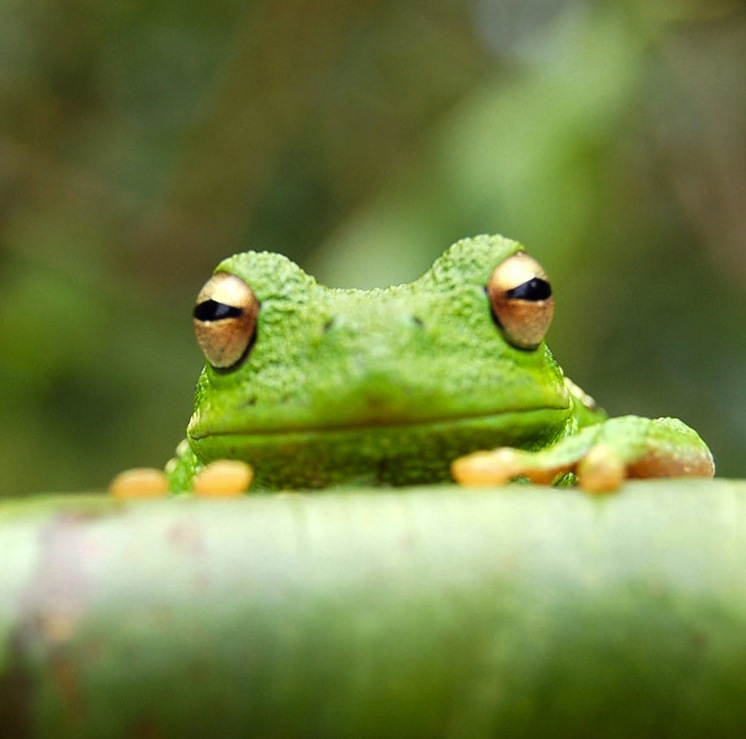
\includegraphics[width=0.5\linewidth]{Figuras/frog.jpg}
    \caption{Diagrama de Casos de Uso}
    \label{casos_de_uso}
\end{figure}

\subsubsection{Dicionário de Casos de Uso}

O \autoref{dicionario_casos_uso} apresenta os dicionários de casos de uso, dos quais apresentam com detalhes cada caso de uso, atores que participam e dão uma descrição deles.

\subsection{Prototipagem}

\section{POC}

A Prova de Conceito (\textit{Proof of Concept} (PoC)) que deve demonstrar a aderência das tecnologias escolhidas com a aplicação que deve ser desenvolvida. Essa prova de conceito deve demonstrar a comunicação desde o usuário até a base de dados e utilizar de forma simples as tecnologias escolhidas para demonstrar que
elas funcionam para o objetivo desejado.

\section{MVP}

O termo MVP foi popularizado por  \citeonline{ries2011lean}, onde ele descreve o conceito como segue:

"O MVP é o menor conjunto de recursos que permite que o empreendedor comece o processo de aprendizado com o mínimo de esforço e o máximo de aprendizado validado sobre os clientes."

Outro autor importante na área, \citeonline{blank2013startup}, define o MVP como:

"Uma ferramenta para testar hipóteses de negócios e iniciar o aprendizado, coletando o máximo de informações validadas sobre os clientes com o menor esforço possível."


% ---
% Finaliza a parte no bookmark do PDF, para que se inicie o bookmark na raiz
% ---
\bookmarksetup{startatroot}% 
% ---

% ---
% Conclusão
% ---
\section{Considerações finais}


De acordo com \citeonline{severino2016metodologia}, na seção de considerações finais o autor tem a oportunidade de fazer uma síntese dos principais pontos abordados e apresentar suas considerações finais sobre o assunto. Embora não haja uma estrutura fixa, existem algumas diretrizes comuns para escrever essa seção.

A seguir, algumas orientações gerais, para complementar a explicação:

1. Recapitule os principais pontos: Na seção de considerações finais, você pode revisitar os principais pontos discutidos ao longo do trabalho e resumir os resultados obtidos. É uma oportunidade para destacar a relevância do estudo e como ele contribui para o conhecimento existente.

2. Discuta as implicações dos resultados: Nessa seção, você pode discutir as implicações práticas e teóricas dos resultados do seu trabalho. 

3. Faça uma reflexão crítica: Use a seção de considerações finais para fazer uma reflexão crítica sobre as limitações do estudo e possíveis viéses. Discuta as dificuldades encontradas, bem como eventuais lacunas de conhecimento que podem ser exploradas por estudos futuros.

4. Encerre de forma concisa e impactante: Finalize a seção de considerações finais com uma frase ou parágrafo que resuma as principais conclusões e destaque a importância do estudo. É uma oportunidade para deixar uma impressão duradoura nos leitores.

% ----------------------------------------------------------
% ELEMENTOS PÓS-TEXTUAIS
% ----------------------------------------------------------
\postextual

% ----------------------------------------------------------
% Referências bibliográficas
% ----------------------------------------------------------

% ----------------------------------------------------------
% Glossário
% ----------------------------------------------------------
%
% Há diversas soluções prontas para glossário em LaTeX. 
% Consulte o manual do abnTeX2 para obter sugestões.
%
% \glossary
% ----------------------------------------------------------
% Apêndices
% ----------------------------------------------------------

\bibliography{referencias}
% ---
% Inicia os apêndices
% ---
\newpage
\begin{apendicesenv}

% % % % ----------------------------------------------------------
\chapter{Requisitos Funcionais}

\begin{longtblr}[
  label = requisitos_f,
  entry = none,
]{
  vline{1-4} = {-}{},
  hline{-} = {1-3}{},
}
Código & Categoria    & Descrição                                                                                       &  \\
RF01   & Cadastro     & {Cadastrar paciente: dados pessoais \\(nome, CPF, data de nascimento, endereço, contato, etc.)} &  \\
RF02   & Paciente     & {Visualizar perfil do paciente: \\histórico de atendimentos e tratamentos}                      &  \\
RF03   & Paciente     & Editar e atualizar dados do paciente                                                            &  \\
RF04   & Cadastro     & {Excluir cadastro de paciente: \\mas mantendo o histórico arquivado}                            &  \\
RF05   & Consulta     & {Agendar nova consulta: \\paciente, profissional, data, hora e local}                           &  \\
RF06   & Consulta     & {Listar consultas agendadas:\\~com filtros por data, profissional ou paciente}                  &  \\
RF07   & Consulta     & {Editar ou cancelar consulta: \\antes da data marcada}                                          &  \\
RF08   & Atendimento  & {Registrar atendimento: \\diagnóstico, conduta, recomendações, etc}                             &  \\
RF09   & Notificação  & {Emitir alertas ou notificações:\\~consultas futuras}                                           &  \\
RF10   & Tratamento   & {Criar plano de tratamento: \\associado a um paciente e diagnóstico}                            &  \\
RF11   & Tratamento   & {Listar tratamentos em andamento,\\concluídos ou cancelados (tipo kanban)}                      &  \\
RF12   & Tratamento   & {Registrar evolução do tratamento: \\observações por etapa ou sessão}                           &  \\
RF13   & Tratamento   & {Anexar prescrições médicas: \\laudos, imagens ou documentos ao tratamento}                     &  \\
RF14   & Relatório    & {Gerar relatórios de acompanhamento:\\paciente, profissional ou período}                        &  \\
RF15   & Histórico    & {Visualizar histórico de consultas: \\evolução clínica}                                         &  \\
RF16   & Exportação   & {Exportar dados: \\PDF, Excel ou outro formato}                                                 &  \\
RF17   & Autenticação & {Autenticar usuários: \\login e senha}                                                          &  \\
RF18   & Permissão    & {Gerenciar permissões: \\admin, profissional de saúde, recepcionista, etc}                      &  \\
RF19   & Log          & {Registrar logs de acesso:\\operações críticas (como edições e exclusões)}                      &  \\
RF20   & Pesquisa     & {Pesquisar pacientes, consultas e tratamentos:\\múltiplos critérios}                            &  \\
RF21   & Filtro       & Aplicar filtros e ordenações nas pesquisas                                                      &  
\end{longtblr}


\chapter{Requisitos Não Funcionais}

\begin{longtblr}[
  label = requisitos_nf,
  entry = none,
]{
  vline{1-4} = {-}{},
  hline{-} = {1-3}{},
}
Código & Categoria       & Descrição                                                                                                               &  \\
RNF01  & Segurança       & {Criptografia de dados sensíveis: \\como senhas e informações médicas}                                                  &  \\
RNF02  & Acesso          & {Controle de acesso baseado em \\perfis de usuário: admin ou cuidador.}                                                 &  \\
RNF03  & Sessão          & {Validação de sessão com expiração \\automática por inatividade}                                                        &  \\
RNF04  & Backup          & {Backups regulares e automáticos: \\para recuperação de dados}                                                          &  \\
RNF05  & Desempenho      & {O sistema deve responder às \\requisições em até 5 segundos \\nas operações}                                           &  \\
RNF06  & Concorrência    & {Suportar múltiplos acessos simultâneos \\sem perda de desempenho}                                                      &  \\
RNF07  & Interface       & {Interface intuitiva e acessível para \\usuários não técnicos}                                                          &  \\
RNF08  & Design          & {Uso de padrões de design \\consistentes e amigáveis}                                                                   &  \\
RNF09  & Manutenção      & {O código-fonte deve ser modular \\e documentado, facilitando a manutenção}                                             &  \\
RNF10  & Arquitetura     & Uso de arquitetura escalável                                                                                            &  \\
RNF11  & Disponibilidade & {O sistema deve estar disponível \\pelo menos 99,5\% do tempo}                                                          &  \\
RNF12  & Integridade     & {Deve garantir integridade dos dados \\em operações simultâneas}                                                        &  \\
RNF13  & Recuperação     & {Deve ser capaz de recuperar-se \\de falhas sem perda de dados}                                                         &  \\
RNF15  & Ambientes       & {Ambientes separados para produção, \\testes e homologação}                                                             &  \\
RNF16  & Segurança       & {O sistema deve exigir autenticação de usuário\\~para qualquer operação de inserção, \\alteração ou exclusão de dados.} &  
\end{longtblr}


\chapter{Regras de Negócio}

\begin{longtblr}[
  label = regras_negocio,
  entry = none,
]{
  vline{1-4} = {-}{},
  hline{-} = {1-3}{},
}
Código & Categoria                      & Descrição                                                                                                                               &  \\
RN01   & Cadastro                       & {Apenas usuários com permissão de cuidador ou \\administrador podem cadastrar dependentes.}                                             &  \\
RN02   & Cadastro                       & {Cada dependente deve ter um \\CPF único e válido no sistema.}                                                                          &  \\
RN03   & Cadastro                       & {O sistema deve impedir o cadastro de dependentes \\com dados incompletos obrigatórios \\(ex: nome, CPF, data de nascimento, contato).} &  \\
RN04   & Cadastro                       & {A exclusão de um dependente não deve arquivar \\todo o histórico, porém não há \\remoção definitiva do banco de dados.}                &  \\
RN05   & Cadastro                       & {A edição de dados sensíveis (como CPF) \\deve ser registrada em log de auditoria.}                                                     &  \\
RN06   & Consultas                      & {Consultas só podem ser agendadas \\para dependentes cadastrados no sistema.}                                                           &  \\
RN07   & Consultas                      & {O sistema deve impedir agendamento\\de duas consultas no mesmo \\horário para o mesmo dependente.}                                     &  \\
RN08   & Consultas                      & {Consultas só podem ser editadas ou \\canceladas antes da data e hora marcadas.}                                                        &  \\
RN09   & Logs                           & {A edição ou exclusão de uma consulta\\criada deve ser registrada em log}                                                               &  \\
RN10   & Tratamentos                    & {Cada tratamento deve estar vinculado a um \\dependente específico e seu diagnóstico.}                                                  &  \\
RN11   & Tratamentos                    & {A evolução de um tratamento deve ser registrada \\com data, cuidador responsável e observações.}                                       &  \\
RN12   & Tratamentos                    & {Prescrições médicas devem ser anexadas com\\extensão válida (PDF, JPG, PNG, etc) \\e tamanho máximo pré-definido.}                     &  \\
RN13   & Tratamentos                    & {Um tratamento só pode ser concluído \\ou cancelado por cuidadores\\com permissão e deve ser registrado em log.}                        &  \\
RN14   & Autenticação                   & {Todos os usuários devem possuir credenciais\\únicas (login e senha criptografados).}                                                   &  \\
RN15   & Autenticação                   & {O acesso ao sistema deve ser restrito por perfis: \\administrador/cuidador.}                                                           &  \\
RN16   & Autenticação                   & {Registros sensíveis só podem\\ser manuseados por perfis autorizados.}                                                                  &  \\
RN17   & Manuseio e exportação de dados & {Toda ação crítica (edição, exclusão, exportação)\\deve ser registrada com data, \\hora, usuário e tipo de operação.}                   &  \\
RN18   & Manuseio e exportação de dados & {O sistema deve permitir pesquisas por \\múltiplos critérios combinados nas filtragens.}                                                &  \\
RN19   & Manuseio e exportação de dados & {Os relatórios devem permitir filtros por \\dependente, período e/ou tratamento.}                                                       &  \\
RN20   & Interface                      & {Toda ação do sistema deve retornar \\mensagem clara de sucesso ou erro.}                                                               &  \\
RN21   & Interface                      & {Listagens com mais de 20 itens devem \\utilizar paginação ou lazy loading.}                                                            &  \\
RN22   & Interface                      & {O sistema deve ser acessível e \\compatível com dispositivos móveis.}                                                                  &  \\
RN23   & Desenvolvimento e Manutenção   & {O código deve ser modular e seguir \\boas práticas de engenharia de software.}                                                         &  \\
RN24   & Desenvolvimento e Manutenção   & {Toda funcionalidade deve prever \\testes automatizados (testes unitários).}                                                            &  
\end{longtblr}

\chapter{Dicionário de Casos de Uso\label{dicionario_casos_uso}}

\begin{longtblr}[
  label = {Manter_Perfil},
  entry = none,
  caption = {Manter Perfil},
]{
  vline{1} = {-}{},
  vline{2} = {-}{},
  vline{3} = {-}{},
  hline{-} = {1-3}{},
  width = \textwidth,
  colspec = {X[2,l] X[8,l]},
}
\textbf{Caso de Uso} & \textbf{Manter Perfil} \\
\textbf{Descrição} & Permite ao cuidador(a) visualizar e editar suas informações pessoais. \\
\textbf{Ator} & Cuidador(a) \\
\textbf{Pré-condições} & Estar autenticado (logado) \\
\textbf{Fluxo Principal} & 1. Cuidador acessa a seção de configuração do perfil \newline 2. Visualiza os dados cadastrados \newline 3. Edita os registros de cuidador \\
\textbf{Extensões} & N/A \\
\textbf{Pós-condição} & Dados do perfil atualizado com sucesso \\
\end{longtblr}

\begin{longtblr}[
  label = {Manter_Dependentes},
  entry = none,
  caption = {Manter Dependentes},
]{
  vline{1} = {-}{},
  vline{2} = {-}{},
  vline{3} = {-}{},
  hline{-} = {1-3}{},
  width = \textwidth,
  colspec = {X[2,l] X[8,l]},
}
\textbf{Caso de Uso} & \textbf{Manter Dependentes} \\
\textbf{Descrição} & Permite ao cuidador(a) adicionar, visualizar, editar e excluir dados de dependentes. \\
\textbf{Ator} & Cuidador(a) \\
\textbf{Pré-condições} & Estar autenticado (logado) \\
\textbf{Fluxo Principal} & 1. Cuidador acessa a seção de configuração do perfil \newline 2. Visualiza os dados dos dependentes \newline 3. Edita ou remove os dados dos dependentes \\
\textbf{Extensões} & N/A \\
\textbf{Pós-condição} & Dados do perfil atualizado com sucesso \\
\end{longtblr}

\begin{longtblr}[
  label = {Agendar_Consulta},
  entry = none,
  caption = {Agendar Consulta},
]{
  vline{1} = {-}{},
  vline{2} = {-}{},
  vline{3} = {-}{},
  hline{-} = {1-3}{},
  width = \textwidth,
  colspec = {X[2,l] X[8,l]},
}
\textbf{Caso de Uso} & \textbf{Agendar Consulta} \\
\textbf{Descrição} & Cuidador(a) agendar consultas para os dependentes. \\
\textbf{Ator} & Cuidador(a) \\
\textbf{Pré-condições} & Estar autenticado (logado) \\
\textbf{Fluxo Principal} & 1. Cuidador acessa a funcionalidade de agendamento \newline 2. Selecionar data e horário \newline 3. Adicionar apelido \newline 4. Confirma o agendamento \\
\textbf{Extensões} & Adicionar ao Google Calendar ou integrar ao calendário do dispositivo utilizado via arquivo .ics\textless\textless extend\textgreater\textgreater \newline Gerar relatório \textless\textless extend\textgreater\textgreater \\
\textbf{Pós-condição} & Consulta agendada e registrada no sistema \\
\end{longtblr}

\begin{longtblr}[
  label = {Gerenciar_Medicacoes},
  entry = none,
  caption = {Gerenciar Medicações do Dependente},
]{
  vline{1} = {-}{},
  vline{2} = {-}{},
  vline{3} = {-}{},
  hline{-} = {1-3}{},
  width = \textwidth,
  colspec = {X[2,l] X[8,l]},
}
\textbf{Caso de Uso} & \textbf{Gerenciar medicações do dependente} \\
\textbf{Descrição} & Permite ao cuidador visualizar, atualizar e acompanhar o uso dos medicamentos de um dependente, incluindo o estoque e registros de consumo. \\
\textbf{Ator} & Cuidador(a) \\
\textbf{Pré-condições} & Estar autenticado (logado) \\
\textbf{Fluxo Principal} & 1. Acessar módulo de medicações \newline 2. Visualizar dados de cada medicamento \newline 3. Registrar consumo \newline 4. Atualizar estoque disponível \\
\textbf{Extensões} & Calcular índice de adesão ao tratamento \textless\textless extend\textgreater\textgreater \newline Exibir alertas de baixo estoque \textless\textless extend\textgreater\textgreater \newline Redirecionar para busca de preços e disponibilidade \textless\textless extend\textgreater\textgreater \\
\textbf{Pós-condição} & Dados dos medicamentos atualizados; adesão e estoque recalculados. \\
\end{longtblr}

\begin{longtblr}[
  label = {Visualizar_Analises_Medicamentos},
  entry = none,
  caption = {Visualizar Análises de Uso de Medicamentos},
]{
  vline{1} = {-}{},
  vline{2} = {-}{},
  vline{3} = {-}{},
  hline{-} = {1-3}{},
  width = \textwidth,
  colspec = {X[2,l] X[8,l]},
}
\textbf{Caso de Uso} & \textbf{Visualizar análises de uso de medicamentos} \\
\textbf{Descrição} & Exibe gráficos e indicadores sobre o uso dos medicamentos, como frequência, horários, aderência e possíveis anomalias. \\
\textbf{Ator} & Cuidador(a) \\
\textbf{Pré-condições} & Estar autenticado (logado) \\
\textbf{Fluxo Principal} & 1. Acessar seção de análises de medicação \newline 2. Visualizar gráficos com dados de uso \\
\textbf{Extensões} & N/A \\
\textbf{Pós-condição} & Gráficos e relatórios exibidos com base nos dados registrados. \\
\end{longtblr}

\begin{longtblr}[
  label = {Observar_Analise_Medicacao},
  entry = none,
  caption = {Observar Análise de Medicação},
]{
  vline{1} = {-}{},
  vline{2} = {-}{},
  vline{3} = {-}{},
  hline{-} = {1-3}{},
  width = \textwidth,
  colspec = {X[2,l] X[8,l]},
}
\textbf{Caso de Uso} & \textbf{Observar análise de medicação} \\
\textbf{Descrição} & Permite ao cuidador(a) visualizar e gerenciar as informações associadas aos tratamentos dos dependentes, como informações gerais, categorização e análise por uso e disponibilidade através de gráficos. \\
\textbf{Ator} & Cuidador(a) \\
\textbf{Pré-condições} & Estar autenticado (logado) \\
\textbf{Fluxo Principal} & 1. Cuidador acessa a seção de medicações \newline 2. Visualiza as análises e informações sobre os medicamentos. \\
\textbf{Extensões} & Permite a geração de relatórios \textless\textless extends\textgreater\textgreater \newline Alterar as informações de gráficos através de filtros \textless\textless extends\textgreater\textgreater \\
\textbf{Pós-condição} & Dados de um tratamento do dependente visualizados com sucesso \\
\end{longtblr}

\begin{longtblr}[
  label = {Controlar_Registros},
  entry = none,
  caption = {Controlar Registros},
]{
  vline{1} = {-}{},
  vline{2} = {-}{},
  vline{3} = {-}{},
  hline{-} = {1-3}{},
  width = \textwidth,
  colspec = {X[2,l] X[8,l]},
}
\textbf{Caso de Uso} & \textbf{Controlar Registros} \\
\textbf{Descrição} & Permite que o administrador realize o controle de usuários e atualizações ao sistema (excluir cuidadores caso haja mau uso, corrigir erros…) \\
\textbf{Ator} & Administrador \\
\textbf{Pré-condições} & Acessar com credenciais de administrador \\
\textbf{Fluxo Principal} & 1. O sistema monitora ações do cuidador. \newline 2. Registra alterações ou eventos automaticamente. \newline 3. Atualiza banco de dados conforme necessário. \\
\textbf{Extensões} & Editar dados do cuidador \textless\textless extend\textgreater\textgreater \newline Editar dados dos dependente \textless\textless extend\textgreater\textgreater \newline Excluir registros \textless\textless extend\textgreater\textgreater \\
\textbf{Pós-condição} & Registros atualizados e armazenados corretamente pelo sistema. \\
\end{longtblr}

\begin{longtblr}[
  label = {Visualizar_Relatorios},
  entry = none,
  caption = {Visualizar Relatórios},
]{
  vline{1} = {-}{},
  vline{2} = {-}{},
  vline{3} = {-}{},
  hline{-} = {1-3}{},
  width = \textwidth,
  colspec = {X[2,l] X[8,l]},
}
\textbf{Caso de Uso} & \textbf{Visualizar Relatórios} \\
\textbf{Descrição} & Permite ao cuidador(a) gerar relatórios de adesão ao tratamento e resultados de consultas. \\
\textbf{Ator} & Cuidador(a) \\
\textbf{Pré-condições} & Estar autenticado (logado) \\
\textbf{Fluxo Principal} & 1. Acessar a seção de relatórios \newline 2. Selecionar o tipo de relatório \newline 3. Gerar e exportar relatório \\
\textbf{Extensões} & Aplicar filtros por período \textless\textless extend\textgreater\textgreater \\
\textbf{Pós-condição} & Relatório gerado e disponível para download \\
\end{longtblr}

\end{apendicesenv}

% % ----------------------------------------------------------
% % Anexos
% % ----------------------------------------------------------
% \cftinserthook{toc}{AAA}
% % ---
% % Inicia os anexos
% % ---
% %\anexos
% \newpage
% \begin{anexosenv}

% % ---
% \chapter{Cras non urna sed feugiat cum sociis natoque penatibus et magnis dis
% parturient montes nascetur ridiculus mus}
% % ---

% Anexos são os documentos não elaborados pelo autor, que servem de fundamentação, comprovação ou ilustração, como mapas, leis, estatutos etc.

% Os apêndices devem aparecer após as referências, e os anexos, após os apêndices.

% \end{anexosenv}

\end{document}
